%!TEX root =  ../Report.tex
\subsection{Classifiers}

%Classification on the combined set of features was conducted against three classifier models, Random Forest (RF), XGBoost and K-Nearest Neighbour (KNN).

\subsubsection{Random Forest}
\label{sec:RF}

In an attempt to find optimal parameters, GridSearchCV and RandomizedSearchCV were utilised. However, due to memory issues on both machines and frequent system crashes due to insufficient memory, experimentation for the Random Forest Classifier instead follows an exploratory approach, using both prior knowledge and iterative testing to create a series of models which were subsequently evaluated and optimised. The training was conducted on both the M2 and VM testbeds. Table \ref{tab:rf-params} details the set of parameters focused on during experimentation, using performance feedback and the model's behaviour on the dataset, these were tweaked and fine-tuned to help enhance the model's performance. Table \ref{tab:rf-parameters} documents the parameters used for all models.

\medskip

Initial experimentation began using default parameters without changing or adding any values (Model 0-2). This helped to establish the baseline performance for subsequent comparison and analysis. This initial model achieved high S-CV average scores on the entire dataset. With such high metrics, it was important to ensure modifications made to the model avoided overfitting. 

\medskip

Subsequent experimentation was conducted by using the model's training metrics along with the confusion matrices, classification reports and predictions on the test set. In Models 3 and 5, it was noted that the modification of the \textit{class\_weight} parameter from its default value to \textit{'weighted'} resulted in a decrease in S-CV performance across all metrics, moreover inspecting the metrics on the test set affirms this, with a higher number of misclassifications, but with higher recall and very low precision rates for several classes. 

In the course of the iterative and exploratory phases, it was observed that additional models and future parameter tuning i.e. Models 3-5 all showed negative performance impacts when compared to the baseline model. This indicated that contrary to expectations, using additional parameter values did not increase the performance of this classifier. It was concluded that for the AWID3 dataset and this specific classification problem, the default parameters for the RandomForestClassifier showed superior performance. Subsequently, additional experimentation was concluded at this stage. 

\begin{table}[h]
\centering
\caption{Parameters for Random Forest Classifier}
\label{tab:rf-params}
\begin{tabular}{|l|l|l|}
\hline
\textbf{Parameter} & \textbf{Description} \\ \hline
n\_estimators & The number of trees in the forest\\
criterion & Function to measure the quality of a split.\\
max\_depth & Maximum depth of the tree. \\
min\_samples\_split & Minimum samples required to split an internal node. \\ 
min\_samples\_leaf & Minimum samples required to be at a leaf node. \\
max\_features & Maximum features to consider when splitting. \\
bootstrap & To bootstrap samples when constructing trees \\
class\_weight & Weights associated with classes \\
random\_state & The random seed.\\ \hline
\end{tabular}
\end{table}

% \begin{table}[h]
% \centering
% \caption{RF Model Metrics}
% \label{tab:rf-metrics}
% \begin{tabular}{|l|l|l|l|l|l|l|}
% \hline
% \textbf{Model} & \textbf{Data Subset} & \textbf{Accuracy} & \textbf{Precision} & \textbf{Recall} & \textbf{F1} & \textbf{Time} \\ \hline
% Base & 80\% & 0.997 & 0.955 & 0.882 & 0.916 & 00:02:34:59 \\ \hline
% Base & 100\% & 0.997 & 0.997 & 0.997 & 0.997 & 00:00:30:60 \\ \hline
% \end{tabular}
% \end{table}

%\begin{table}[h]
%\centering
%\caption{RF Evaluation Set Metrics}
%\label{tab:rf-metrics}
%\begin{tabular}{|l|l|l|l|l|l|}
%\hline
%\textbf{Model} & \textbf{Data Size} & \textbf{Accuracy} & \textbf{Precision} & \textbf{Recall} & \textbf{F1}  \\ \hline
%Stock & 80\% & 0.997 & 0.955 & 0.882 & 0.916  \\ \hline
%Stock & 100\% & 0.997 & 0.997 & 0.997 & 0.997 \\ \hline
%\end{tabular}
%\end{table}

\begin{table}[H]
\centering
\caption{RF Model Parameters}
\label{tab:rf-parameters}
\begin{tabular}{llllll}
\hline
Parameter & Model 0-2 & Model 3 & Model 4 & Model 5\\ \hline
n\_estimators: & 100 & 100 & 200 & 100\\
max\_depth: & None & 10 & 15 & 10  \\
min\_samples\_leaf: & 1 & 2 & 1 & 2 \\
min\_samples\_split: & 2 & 3 & 2 & 3 \\
random\_state: & 1234 & 1234 & 1234 & 1234 \\
class\_weight: & None & None & balanced & balanced \\ \hline
\end{tabular}
\end{table}



%\paragraph{Confusion Matrix}
%
%\begin{figure}[H]
%    \centering
%    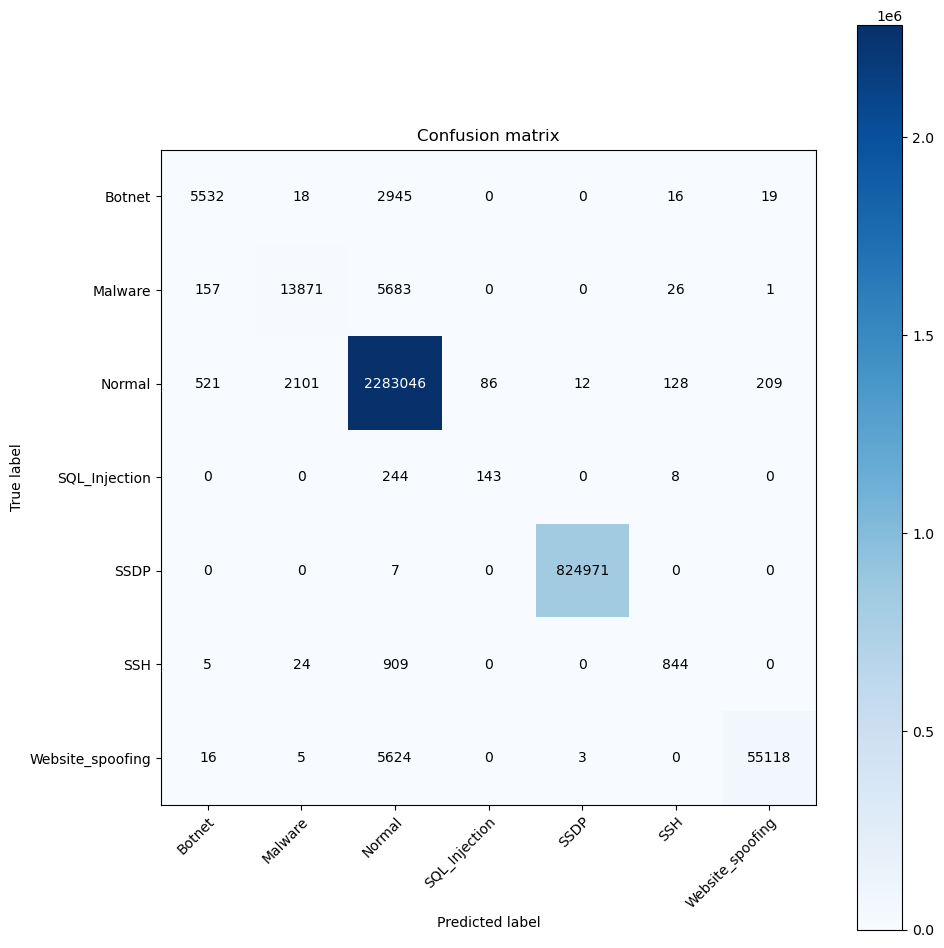
\includegraphics[width=0.85\textwidth]{Appendices/NN Confusion Matrix 3-04-23.png}
%    \caption{RF Confusion Matrix}
%    \label{fig:rf_confusion_matrix}
%\end{figure}
